% !TeX program = pdfLaTeX
\documentclass[12pt]{article}
\usepackage{amsmath}
\usepackage{graphicx,psfrag,epsf}
\usepackage{enumerate}
\usepackage{natbib}
\usepackage{textcomp}
\usepackage[hyphens]{url} % not crucial - just used below for the URL
\usepackage{hyperref}
\providecommand{\tightlist}{%
  \setlength{\itemsep}{0pt}\setlength{\parskip}{0pt}}

%\pdfminorversion=4
% NOTE: To produce blinded version, replace "0" with "1" below.
\newcommand{\blind}{0}

% DON'T change margins - should be 1 inch all around.
\addtolength{\oddsidemargin}{-.5in}%
\addtolength{\evensidemargin}{-.5in}%
\addtolength{\textwidth}{1in}%
\addtolength{\textheight}{1.3in}%
\addtolength{\topmargin}{-.8in}%

%% load any required packages here



% Pandoc citation processing


\begin{document}


\def\spacingset#1{\renewcommand{\baselinestretch}%
{#1}\small\normalsize} \spacingset{1}


%%%%%%%%%%%%%%%%%%%%%%%%%%%%%%%%%%%%%%%%%%%%%%%%%%%%%%%%%%%%%%%%%%%%%%%%%%%%%%

\if0\blind
{
  \title{\bf Supplemental Materials for ``Popuarity Adjusted Block
Models are Generalized Random Dot Product Graphs''}

  \author{
        John Koo \\
    Department of Statistics, Indiana University\\
     and \\     Minh Tang \\
    Department of Statistics, North Carolina State University\\
     and \\     Michael W. Trosset \\
    Department of Statistics, Indiana University\\
      }
  \maketitle
} \fi

\if1\blind
{
  \bigskip
  \bigskip
  \bigskip
  \begin{center}
    {\LARGE\bf Supplemental Materials for ``Popuarity Adjusted Block
Models are Generalized Random Dot Product Graphs''}
  \end{center}
  \medskip
} \fi

\bigskip
\begin{abstract}

\end{abstract}

\noindent%
{\it Keywords:} 
\vfill

\newpage
\spacingset{1.45} % DON'T change the spacing!

\newcommand{\diag}{\mathrm{diag}}
\newcommand{\tr}{\mathrm{Tr}}
\newcommand{\blockdiag}{\mathrm{blockdiag}}
\newcommand{\indep}{\stackrel{\mathrm{ind}}{\sim}}
\newcommand{\iid}{\stackrel{\mathrm{iid}}{\sim}}
\newcommand{\Bernoulli}{\mathrm{Bernoulli}}
\newcommand{\Betadist}{\mathrm{Beta}}
\newcommand{\BG}{\mathrm{BernoulliGraph}}
\newcommand{\PABM}{\mathrm{PABM}}
\newcommand{\RDPG}{\mathrm{RDPG}}
\newcommand{\GRDPG}{\mathrm{GRDPG}}
\newcommand{\Multinomial}{\mathrm{Multinomial}}
\newtheorem{theorem}{Theorem}
\newtheorem{lemma}{Lemma}
\newtheorem{proposition}{Proposition}
\newtheorem{remark}{Remark}
\newtheorem{definition}{Definition}
\newtheorem{example}{Example}

\hypertarget{sparsity-simulation-study}{%
\section{Sparsity Simulation Study}\label{sparsity-simulation-study}}

In this simulation study, we use the same setup as in the simulations
for balanced communities but with fixed \(K = 3\) and \(n = 2^{11}\) and
vary the sparsity parameter \(\rho \in (0, 1]\) (this was fixed at
\(\rho_n = 1\) for the previous simulations. More specifically,

\begin{itemize}
\tightlist
\item
  Number of vertices \(n = 2048\)
\item
  Number of underlying communities \(K = 3\)
\item
  Sparsity parameter \(\rho_n = 0.1, .03, 0.5, 0.7, 0.9\)
\item
  Mixture parameters \(\alpha_k = 1 / K\) for \(k = 1, ..., K\) (i.e.,
  each community label has an equal probability of being drawn)
\item
  Community labels
  \(z_k \stackrel{\mathrm{iid}}{\sim}\mathrm{Multinomial}(\alpha_1, ..., \alpha_K)\)
\item
  Within-group popularities
  \(\lambda^{(kk)} \stackrel{\mathrm{iid}}{\sim}\mathrm{Beta}(2, 1)\)
\item
  Between-group popularities
  \(\lambda^{(k \ell)} \stackrel{\mathrm{iid}}{\sim}\mathrm{Beta}(1, 2)\)
  for \(k \neq \ell\)
\end{itemize}

Fifty simulations were performed for each combination of \(n\) and
\(K\). The results for community detection and parameter estimation
error are shown in Fig. \ref{fig:sparsity_sim}. Community detection
error is defined as the number of misclustered vertices. Parameter
estimation error is defined as \(\frac{1}{n} \|P - \hat{P}\|_F\) where
\(\hat{P}\) is the estimated edge probability matrix.

\begin{figure}[h]

{\centering 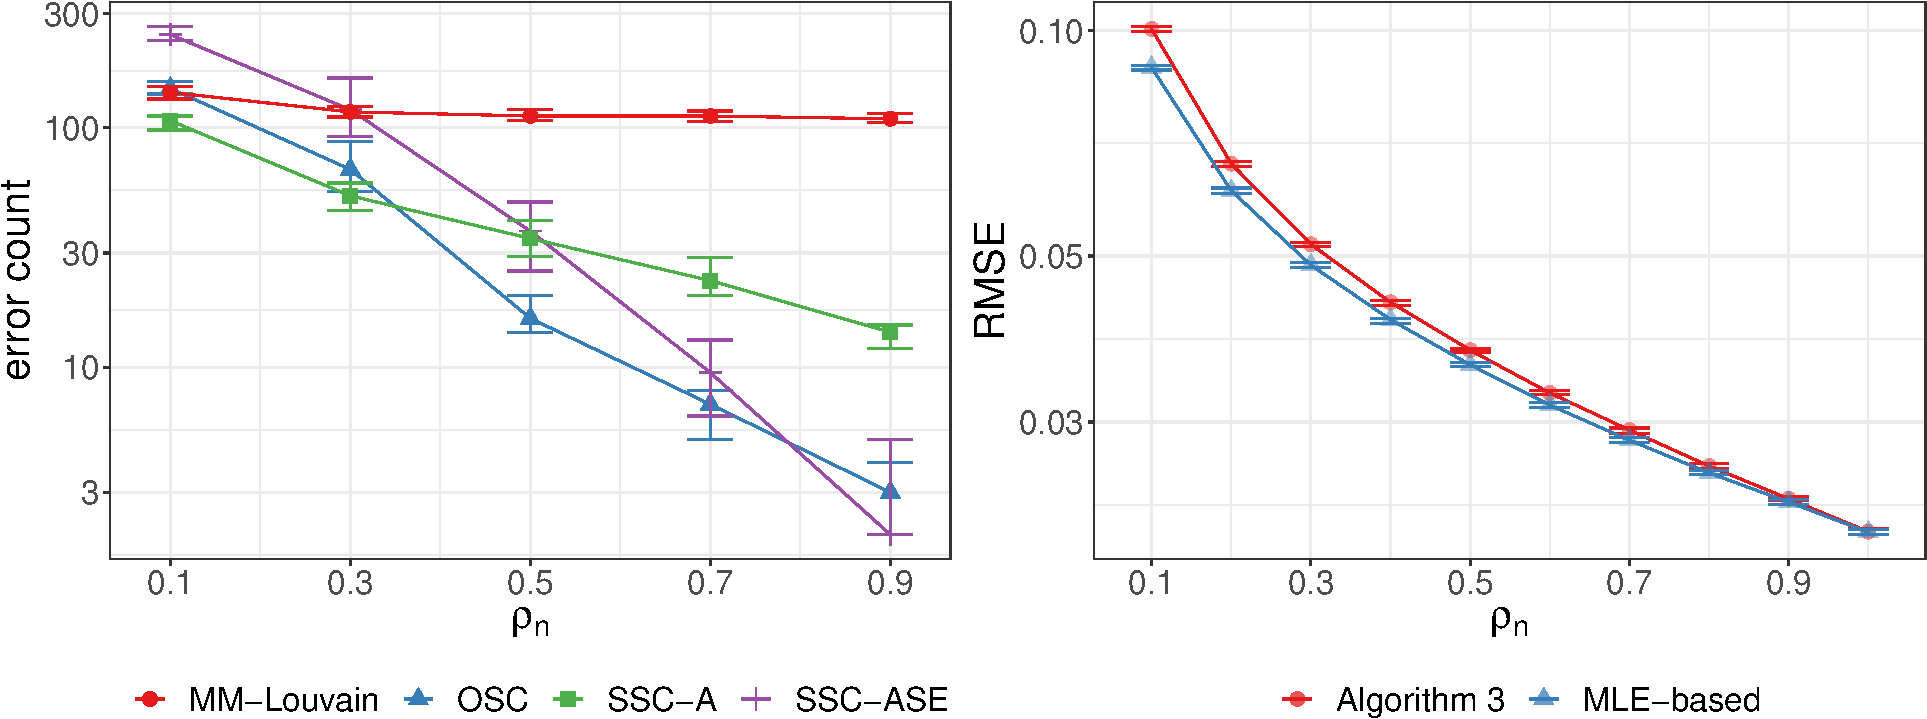
\includegraphics[width=1\linewidth]{sparsity-sim_files/figure-latex/sparsity_sim-1} 

}

\caption{Community detection error counts (left) and popularity parameter RMSEs (right) for $n = 2048$ and $K = 3$ and varying $\rho_n$. Simulations were repeated 50 times for each $\rho_n$.}\label{fig:sparsity_sim}
\end{figure}

\bibliographystyle{agsm}
\bibliography{bibliography.bib}

\end{document}
